Tato kapitola se věnuje návrhu aplikace, tedy technologické architektury celé platformy a jednotlivých implementací, návrhu funkcionalit a uživatelskému rozhraní aplikace. V~následujících sekcích budou rozebírány jednotlivé navržené funkcionality a jejich rozhraní. Nejprve je ale potřeba si stanovit nějaký vzhledový styl aplikace.

Pro návrh uživatelského rozhraní aplikace byl použit nástroj \emph{Figma} \cite{figma}, dále byly použity zdroje z~šablony \emph{Apple Design Resources} \cite{apple-design-resources}.

%---------------------------------------------------------------
\section{Vzhledový styl aplikace}
%---------------------------------------------------------------

Aplikace cílí na platformu iOS, což bude důležitou součástí jejího návrhu. Apple definuje rozsáhlou příručku pro návrh uživatelského rozhraní pro platformu iOS \cite{apple-design-guidelines-ios} a návrh aplikace se touto příručkou bude v~mnoha ohledech řídit.

Každá aplikace má nějaký svůj vzhledový styl, který definuje základní barvy, které bude aplikace používat, vzhledy tlačítek, textových polí, fontů a dalšího. Následující definice těchto prvků vychází převážně z~osobní preference, která se soustředí spíše na jednoduchost a ne příliš velkou výraznost rozhraní. Cílem tedy bude se přiblížit systémovému vzhledu platformy iOS a přidat vlastní mírný vzhledový jazyk.

%---------------------------------------------------------------
\subsection{Barvy}
%---------------------------------------------------------------

Základní návrh barev aplikace lze nahlédnout v~obrázku \ref{fig:colors}. Barvy jsou navrženy tak, aby vždy vznikl dostatečný kontrast mezi barvou pozadí a barvou popředí.

\begin{figure}[h]
	\centering
	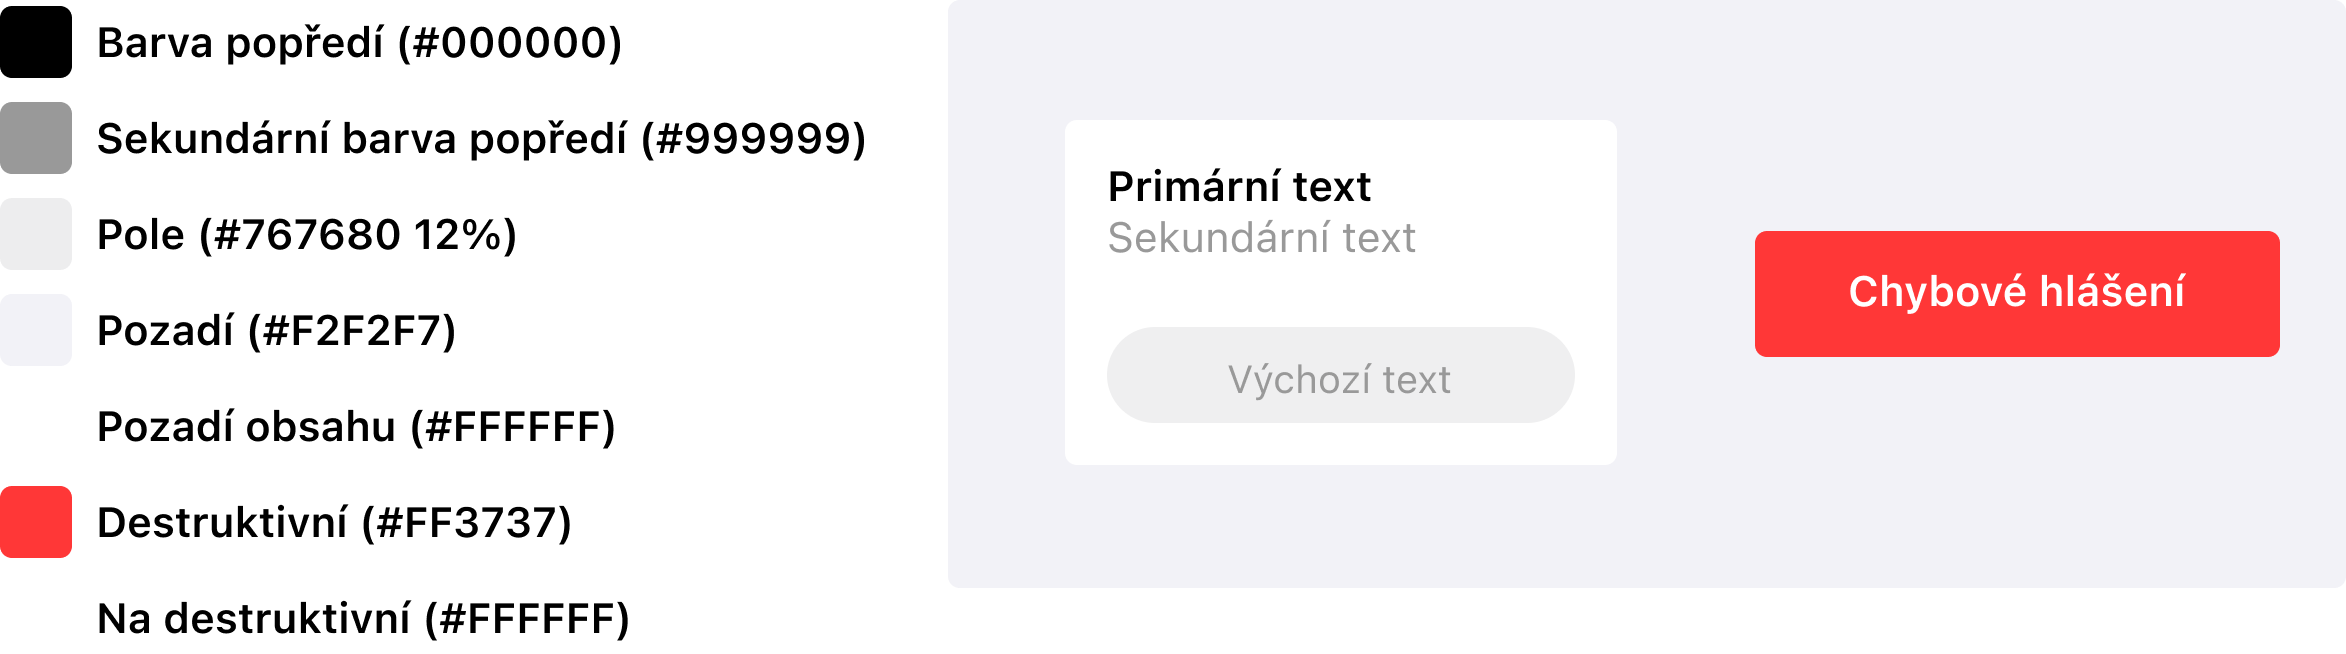
\includegraphics[width=\textwidth]{colors.png}
	\caption{Vzhledový styl aplikace – Barvy}
	\label{fig:colors}
\end{figure}

%---------------------------------------------------------------
\subsection{Fonty}
%---------------------------------------------------------------

Základní návrh fontů lze nahlédnout v~obrázku \ref{fig:fonts}. Daný font bude vždy používat systémovou rodinu fontů, tedy obvykle \emph{San Francisco} (SF). Jednotlivé velikosti jsou pouze referenční, protože aplikace by měla podporovat dynamické fonty a reflektovat tak škálování uživatele. Daná velikost je tedy velikost pro výchozí nastavení škálování textu.

\begin{figure}[h]
	\centering
	
\includegraphics[width=\textwidth]{fonts.png}
	\caption{Vzhledový styl aplikace – Fonty}
	\label{fig:fonts}
\end{figure}

%---------------------------------------------------------------
\subsection{Prvky}
%---------------------------------------------------------------

Návrh prvků rozhraní vychází z~již definovaných barev a fontů, lze jej nahlédnout v~obrázku \ref{fig:elements}.

\begin{figure}[h]
	\centering
	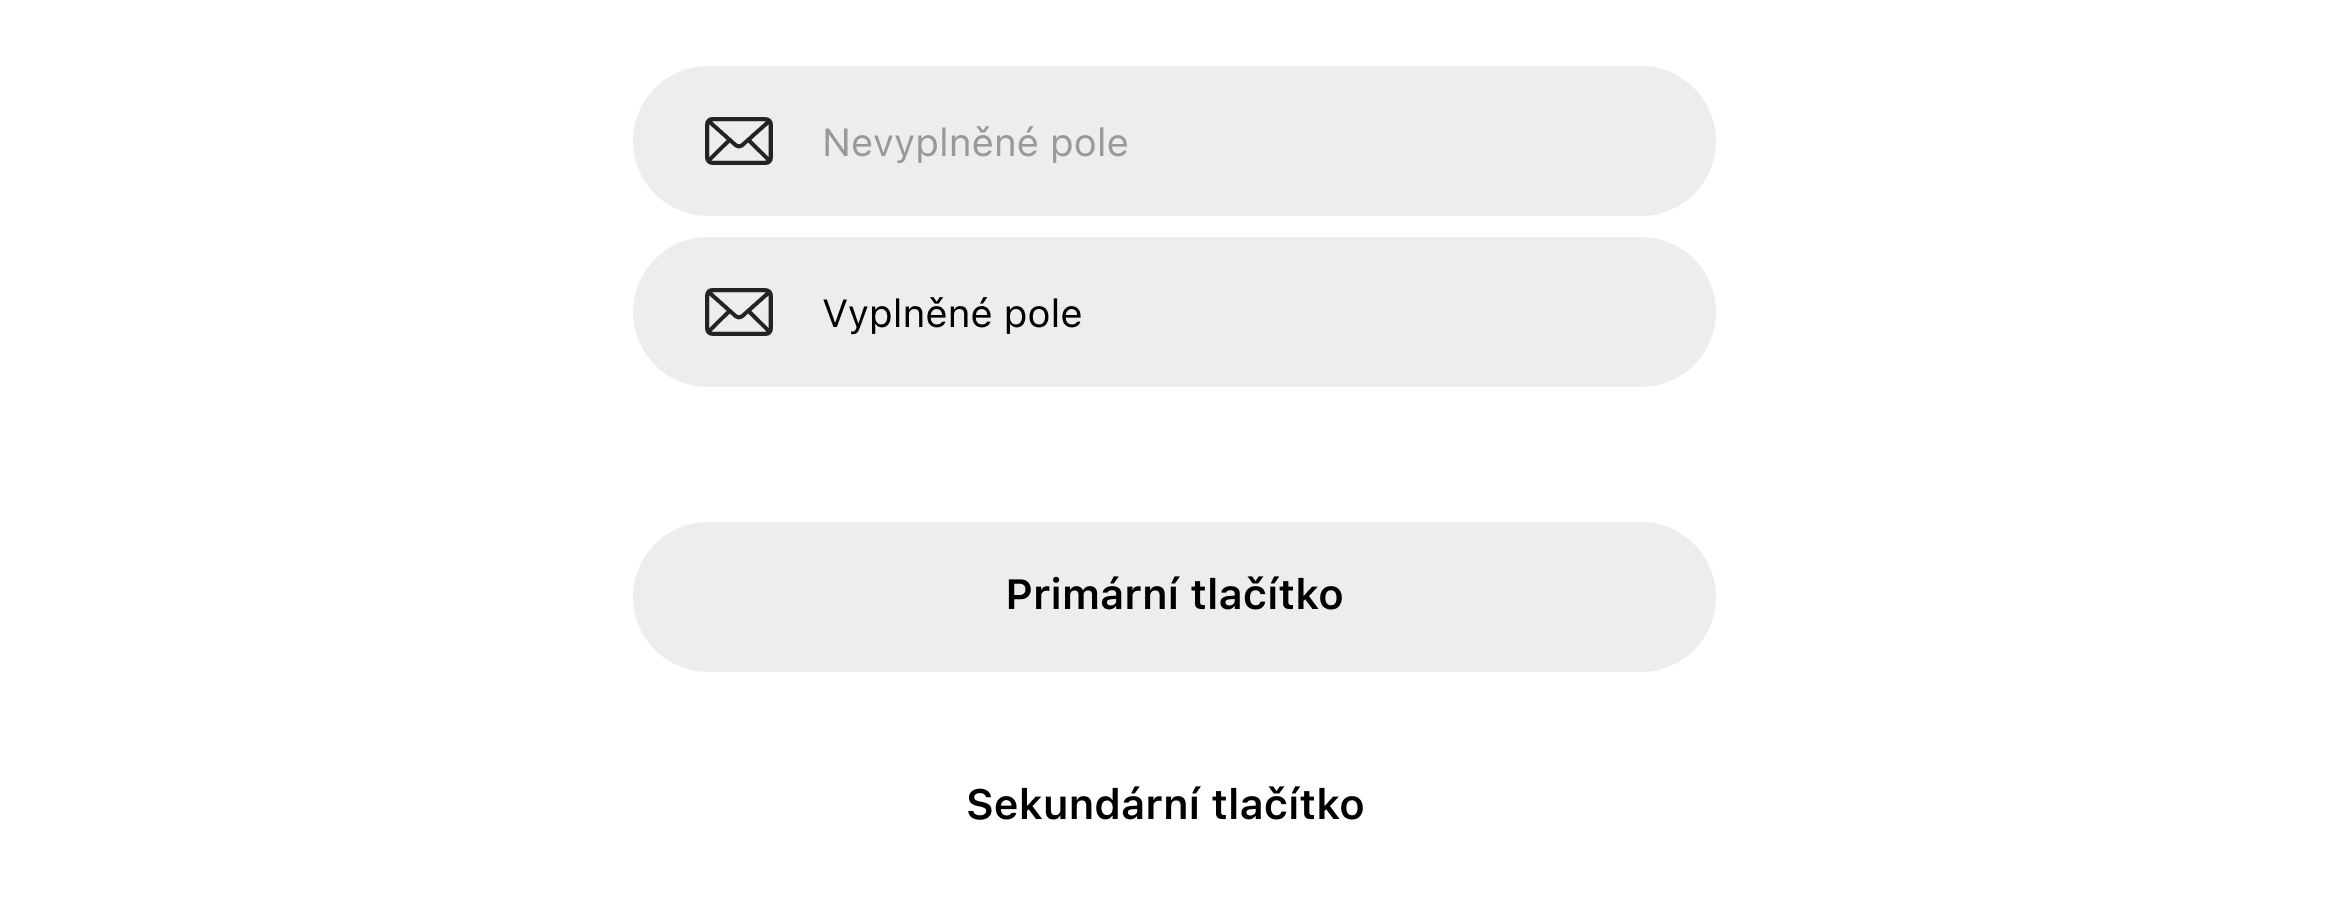
\includegraphics[width=\textwidth]{elements.png}
	\caption{Vzhledový styl aplikace – Prvky}
	\label{fig:elements}
\end{figure}

Na všechny ostatní prvky, jako prvky navigace, seznamy, alerty, a další, bude využito systémových prvků. Tím bude nejlépe vyhověno vzhledové příručce firmy Apple, pouze budou upravné některé barvy těchto prvků, aby ladily k~vzhledu aplikace.

%---------------------------------------------------------------
\subsection{Název a ikona}
%---------------------------------------------------------------

Návrh chytlavého názvu bývá obvykle složitá věc. Pro tuto aplikaci byl zvolen název \emph{Trackee} (anglicky [tra·ki]), který je odvozen z~anglického pojmu \emph{Time tracking}, což představuje měření odpracovaného času. Koncovka \emph{-ee} je také poslední dobou častou volbou pro názvy různorodých aplikací, jako \emph{Spendee} \cite{spendee}, \emph{Fondee} \cite{fondee} a další. Pod tímto názvem není registrována žádná ochranná známka \cite{upd-database}, ani není veden žádný záznam u~správce české domény \cite{cz-nic-trackee}.

Ikona aplikace také neprocházela nijak složitým procesem návrhu, byl pouze použit systémový symbol časovače na pozadí s~barvami aplikace popředí a pole. Ikonku lze nahlédnout v~obrázku \ref{fig:app-icon}.

\begin{figure}[h]
	\centering
	
\includegraphics[width=5cm]{trackee.png}
	\caption{Ikona aplikace}
	\label{fig:app-icon}
\end{figure}

%---------------------------------------------------------------
\section{Funkcionality aplikace a jejich uživatelské rozhraní}
%---------------------------------------------------------------

Aplikace bude primárně sloužit pro zaznamenávání odpracovaného času. Je tedy potřeba, aby každý uživatel měl možnost si vytvářet vlastní záznamy a další data, která budou propojena pouze s~ním, a ke kterým bude mít přístup pouze on. Toto obvyklý případ užití mobilní aplikace, který ze své podstaty vyžaduje nějakou formu vytvoření uživatelského účtu, se kterým budou data propojena, a jeho autentizace. Nejobvyklejším způsobem autentizace je autentizace pomocí e-mailu a hesla. Tento způsob je i~poměrně jednoduchý z~hlediska implementace a spousta poskytovatelů BaaS (Backend as a Service, vizte \ref{baas}) tento způsob autentizace implementuje. 

%---------------------------------------------------------------
\subsection{Přihlášení a registrace}
%---------------------------------------------------------------

Přihlašovací obrazovka bude obsahovat pouze nadpis, pole pro vyplnění e-mailu, hesla, primární tlačítko pro přihlášení a sekundární tlačítko pro registraci. Obrazovka pro registraci, která se otevře po kliku na tlačítko pro registraci, poté bude od uživatele potřebovat také jen e-mail a heslo, které je ale zvykem napsat dvakrát, aby se snížila šance, že se v~něm vyskytl překlep. Obrazovky přihlášení a registrace lze nahlédnout v~obrázku \ref{fig:onboarding}. Úspěšné přihlášení a registrace uživatele přesměruje na hlavní obrazovku aplikace.

\begin{figure}[h]
    \centering
    \begin{subfigure}[b]{0.4\textwidth}
		\centering
		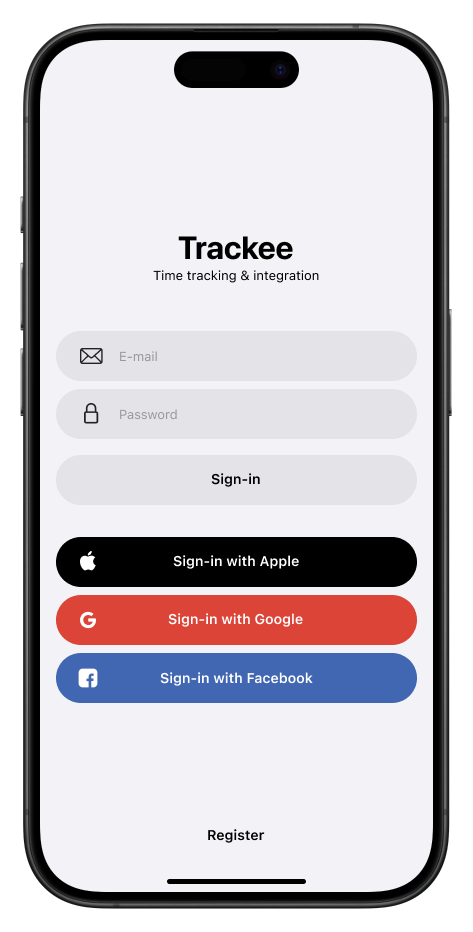
\includegraphics[width=6cm]{login.png}
		\caption{Přihlášení}
		\label{fig:login}
	\end{subfigure}
	\hspace{2cm}
	\begin{subfigure}[b]{0.4\textwidth}
		\centering
		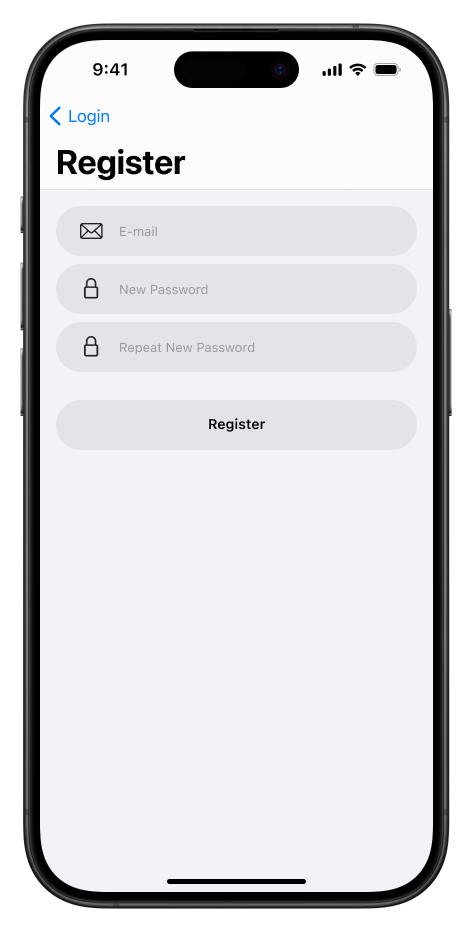
\includegraphics[width=6cm]{register.png}
		\caption{Registrace}
	\end{subfigure}
	\caption{Onboarding}
	\label{fig:onboarding}
\end{figure}

%---------------------------------------------------------------
\subsection{Lišta karet a časovač}
%---------------------------------------------------------------

Navigace mezi hlavními obrazovkami aplikace bude řešena pomocí lišty karet, jelikož se jedná o~častý a doporučený způsob, jak navigovat mezi vzájemně exkluzivními částmi obsahu \cite{apple-guidelines-tabbars}. Hlavní obrazovkou bude přehled, na kterém bude uživatel moct ovládat časovač, a kde uvidí historii svých časových záznamů, seřazenou od nejnovějších po nejstarší. Jelikož pro uživatele je nejjednodušší dosáhnout na ovládací prvky, které jsou ve spodní části displeje, bude ovládání časovače umístěno ve spodní části obrazovky, a časové záznamy se budou řadit nad ním. Návrh této obrazovky lze nahlédnout na obrázku \ref{fig:timer}.

\begin{figure}[h]
    \centering
    \begin{subfigure}[b]{0.4\textwidth}
		\centering
		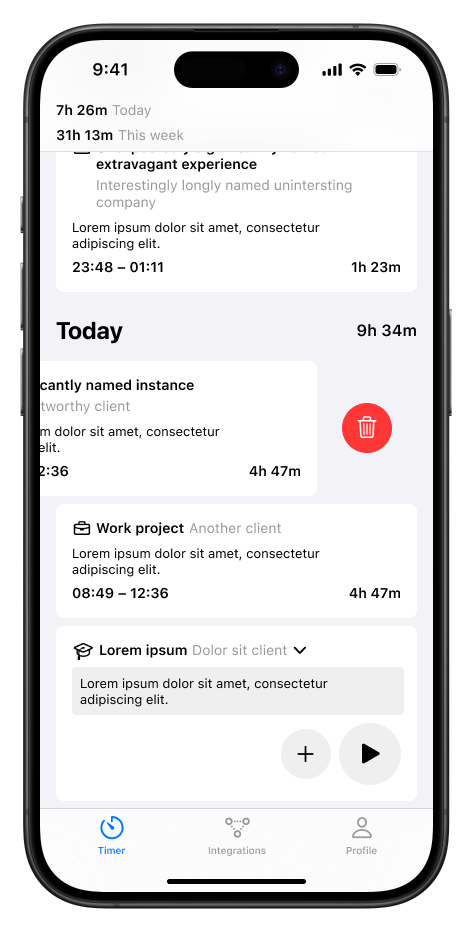
\includegraphics[width=6cm]{timer.png}
		\caption{Časovač}
		\label{fig:timer}
	\end{subfigure}
	\hspace{2cm}
	\begin{subfigure}[b]{0.4\textwidth}
		\centering
		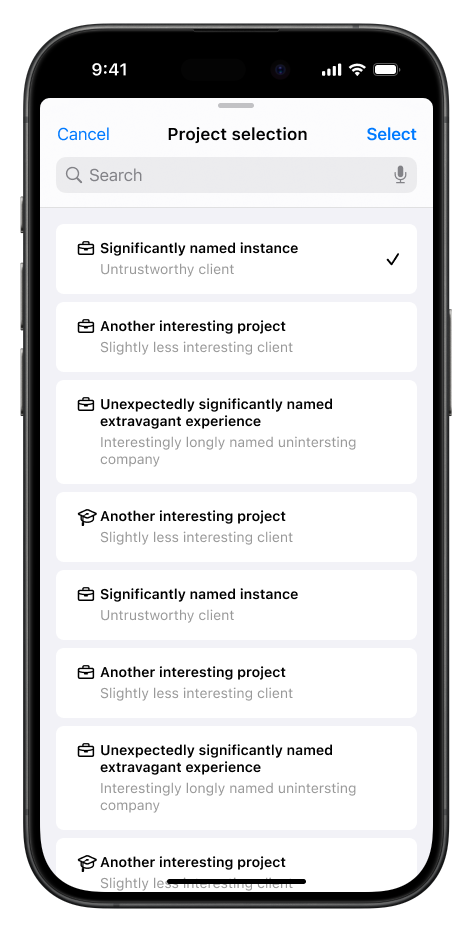
\includegraphics[width=6cm]{project-selection.png}
		\caption{Výběr projektu}
		\label{fig:project-selection}
	\end{subfigure}
	\caption{Hlavní obrazovka}
	\label{fig:timer-and-project-selection}
\end{figure}

Ovládací panel pro časovač může mít různé varianty, jak bude vypadat, podle toho, v~jakém je stavu. Návrh počítá se dvěma možnostmi, jak půjde přidávat časové záznamy do historie:
\begin{itemize}
\item Pomocí časovače – uživatel zapne časovač, když bude chtít začít měření, a poté ho vypne, když bude měření chtít ukončit, čímž se automaticky uloží záznam se zadanými vlastnostmi.
\item Ručně – uživatel ručně zadá začátek a konec záznamu a poté časový záznam uloží.
\end{itemize}
Ovládací panel půjde přepínat mezi těmito dvěma stavy pomocí vedlejšího tlačítka. Hlavní ovládací tlačítko bude vypínat/zapínat časovač, pokud bude přepnut do stavu časovače, nebo bude přidávat ruční záznam, pokud bude v~ručním stavu. V~ovládacím panelu časovače bude také možné vybrat projekt a popis, které budou k~danému záznamu přiděleny. Klik na volbu projektu otevře novou obrazovku, která umožní vyhledávání v~projektech a výběr projektu, jak lze vidět na obrázku \ref{fig:project-selection}. Různé stavy časovače (časovač/manuální, zapnutý/vypnutý, vyplněný/nevyplněný, atd.) lze nahlédnout v~obrázku \ref{fig:timer-control-variants}.

\begin{figure}[h]
	\centering
	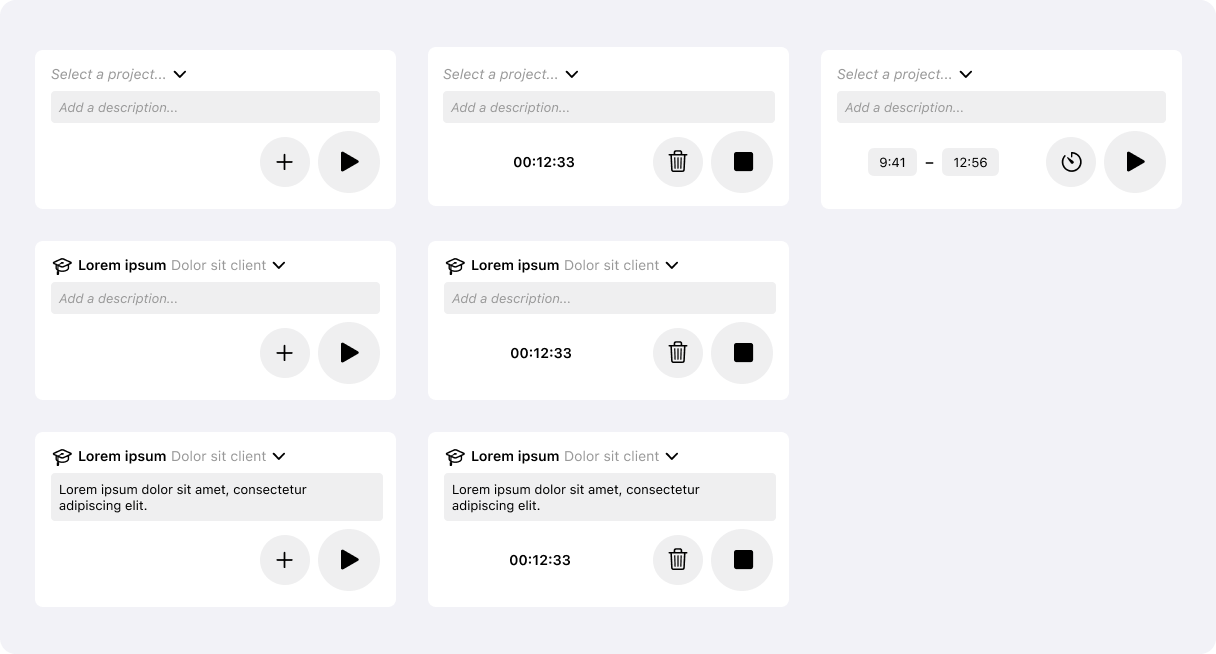
\includegraphics[width=\textwidth]{timer-control-variants.png}
	\caption{Různé stavy ovladače pro časovač}
	\label{fig:timer-control-variants}
\end{figure}

Na obrázku \ref{fig:timer} lze dále v~horní části obrazovky vidět souhrn časových záznam za tento den a týden. Uživatel tak uvidí, kolik času již odpracoval v~daný den i~týden. Časové záznamy v~historii budou také seskupeny podle dnů – každý den bude mít nadpis s~datem a součtem odpracovaného času za ten den. Jednotlivé záznamy také půjdou mazat pomocí posuvného gesta.

Vzhledem k~tomu, že v~historii se může časem nacházet mnoho záznamů, měla by tato obrazovka podporovat stránkování, tedy funkci, že nebude ze zdroje načítat všechny záznamy najednou, ale pouze nějaký kus (stránku), a postupně může načítat další, pokud si to uživatel bude přát. Pokud se během načítání objeví chyba, tak se na této obrazovce ovládací panel časovače ani historie záznamů vůbec nezobrazí – zobrazí se pouze popis chyby a tlačítko pro opakování pokusu o~načtení. Pokud uživatel zatím žádné záznamy mít nebude, tak nebude potřeba zobrazovat nějakou explicitní formu prázdné obrazovky – pouze bude ve spodní části obrazovky ovládací panel a nad tím prázdno.

U~obrazovky pro výběr projektu bude také explicitní chybový stav, který ukáže popis chyby včetně tlačítka pro opakování. Na této obrazovce už ale bude potřeba definovat i~prázdný stav, aby se zobrazila nějaká instrukce, že uživatel nemá vytvořené žádné projekty a musí si je vytvořit na místě k~tomu určeném (bude navrženo dále). Prázdná data lze ale ještě rozdělit do dvou kategorií – prázdná data kvůli tomu, že uživatel žádné projekty nemá, nebo prázdná data kvůli tomu, že jeho vyhledávání neodpovídá žádný projekt. Pro tyto dva stavy je potřeba použít rozdílné texty pro uživatele.

%---------------------------------------------------------------
\subsection{Profil uživatele}
%---------------------------------------------------------------

Poslední kartou v~navigační liště aplikace bude karta s~Profilem. Uživatel zde bude mít základní přehled a akce týkající se jeho účtu, jak lze nahlédnout na obrázku \ref{fig:profile-overview}. Uživatel se odsud dostane do seznamu klientů a seznamu profilů, dále si může pomocí tlačítka svůj účet smazat, nebo se odhlásit, což ho vrátí zpět na přihlašovací obrazovku \ref{fig:login}. Mazání účtu je nevratná akce, která vymaže spoustu dat spojených s~uživatelem, je tedy potřeba alespoň ukázat ověřující dialog, který lze nahlédnout na obrázku \ref{fig:profile-delete}. 

\begin{figure}[h]
    \centering
    \begin{subfigure}[b]{0.4\textwidth}
		\centering
		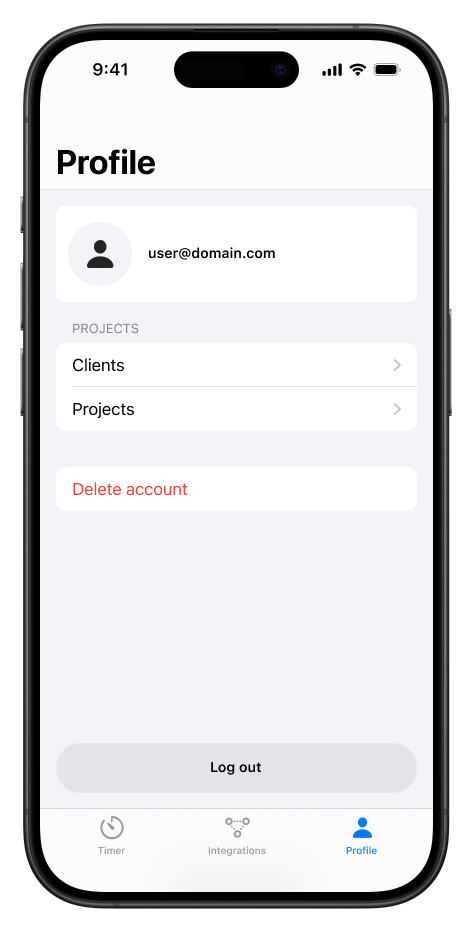
\includegraphics[width=6cm]{profile.png}
		\caption{Přehled}
		\label{fig:profile-overview}
	\end{subfigure}
	\hspace{2cm}
	\begin{subfigure}[b]{0.4\textwidth}
		\centering
		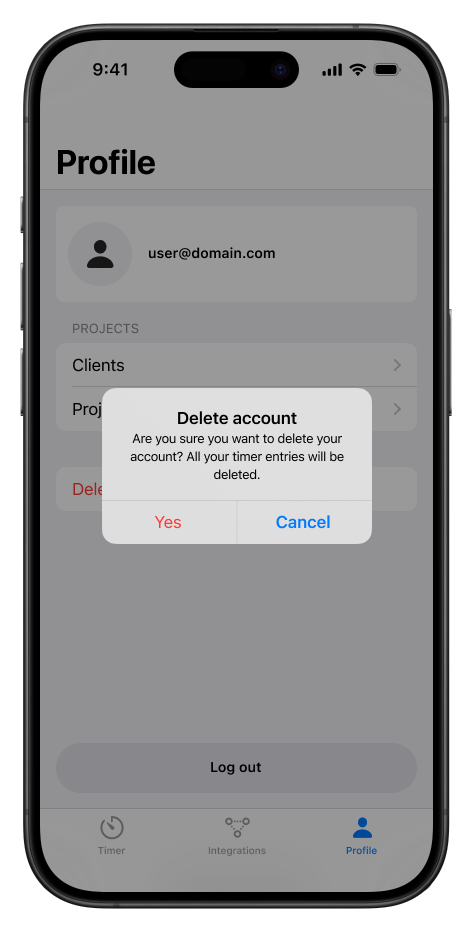
\includegraphics[width=6cm]{profile-delete.png}
		\caption{Smazání účtu}
		\label{fig:profile-delete}
	\end{subfigure}
	\caption{Profil}
	\label{fig:profile}
\end{figure}

V~horní části obrazovky se také nachází uživatelův e-mail, jako indikace toho, na kterém účtě je uživatel přihlášen.

Pokud uživatel klikne na tlačítko klientů, zobrazí se mu seznam jeho klientů, jak lze vidět na obrázku \ref{fig:client-list}. V~tomto seznamu může v~klientech vyhledávat, otevřít detail klienta, nebo vytvořit nového, pomocí tlačítka vpravo nahoře v~navigační liště. Při kliknutí na konkrétního klienta, s~cílem zobrazit jeho detail, i~při kliknutí na volbu tvorby nového klienta, se zobrazí stejná obrazovka detailu, kterou lze nahlédnout na obrázku \ref{fig:new-client}. V~případě zobrazení detailu již existujícího klienta se akorát změní název v~navigační liště a předvyplní se hodnoty klienta. 

Při tvorbě nebo úpravě klienta uživatel může zvolit jeho název. V~budoucnu je možné přidat další parametry, které by mohly být ke klientovi přiděleny. Kliknutím na tlačítko \emph{Uložit} v~navigační liště se upravený klient uloží a uživatel bude odnavigován zpět na seznam klientů. V~případě, že uživatel klikne na tlačítko zrušit, bude také odnavigován zpět na seznam, ale všechny změny budou zahozeny.

Seznam projektů by měl mít také definované stavy pro chybu a prázdná data. V~případě chyby se zobrazí popis chyby a tlačítko pro opakování, v~případě, že uživatel nemá žádné klienty, se zobrazí tato informace a instrukce k~tomu, aby si nějakého klienta vytvořil. Opět je také potřeba rozlišit mezi tím, zda se žádní klienti nezobrazují proto, protože žádní nejsou, nebo protože žádní nevyhovují vyhledávánému výrazu.

Detail klienta bude mít také explicitní chybový stav, ale prázdný stav zde potřeba není, jelikož existující klient musí mít data vždycky, a nový klient určitě žádná nemá, tudíž budou pole prázdná.

\begin{figure}[h]
    \centering
    \begin{subfigure}[b]{0.4\textwidth}
		\centering
		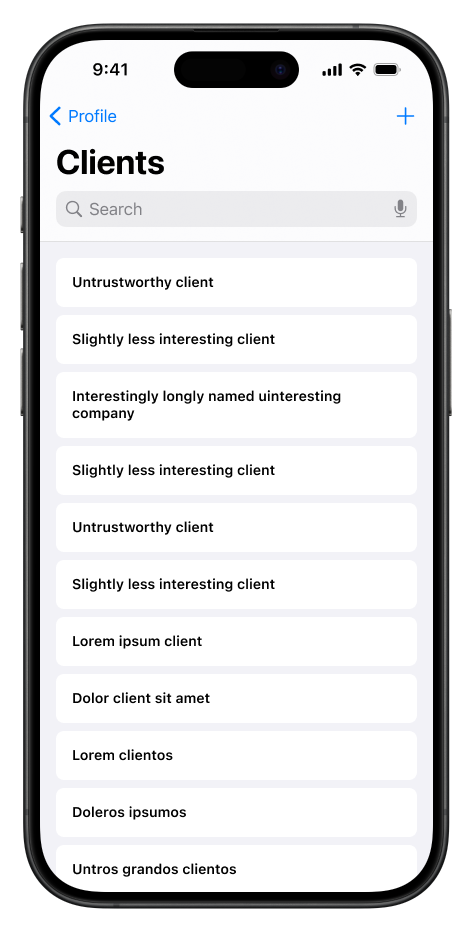
\includegraphics[width=6cm]{clients.png}
		\caption{Seznam}
		\label{fig:client-list}
	\end{subfigure}
	\hspace{2cm}
	\begin{subfigure}[b]{0.4\textwidth}
		\centering
		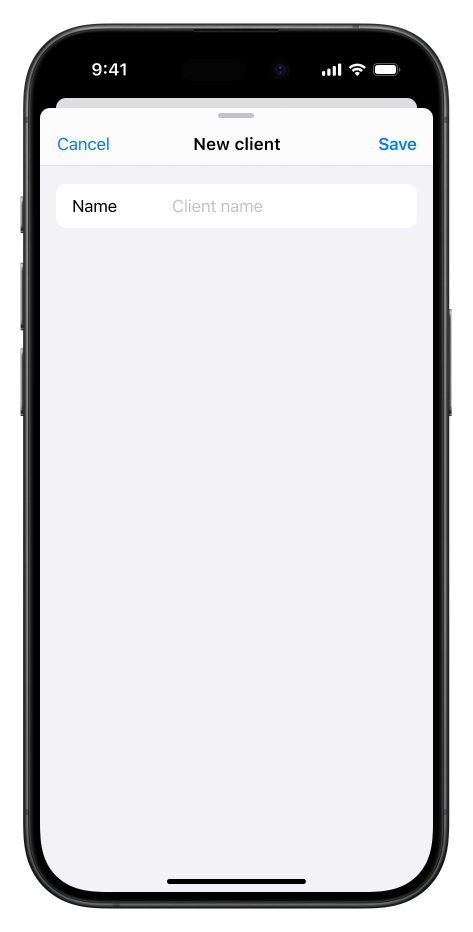
\includegraphics[width=6cm]{new-client.png}
		\caption{Nový klient}
		\label{fig:new-client}
	\end{subfigure}
	\caption{Klienti}
	\label{fig:clients}
\end{figure}

Seznam projektů a detail projektu funguje stejným způsobem, jako u~klientů. Kliknutí na tlačítko projektů v~profilu otevře seznam, odkud lze otevřít detail/tvorbu nového projektu. Seznam projektů lze nahlédnout na obrázku \ref{fig:project-list} a detail projektu na obrázku \ref{fig:new-project}.

Detail projektu narozdíl od klienta obsahuje více informací. Každý projekt musí patřit k~nějakému klientovi, tudíž je potřeba tohoto klienta zvolit, k~čemuž bude sloužit další obrazovka pro výběr klienta, která bude vypadat stejně, jako seznam klientů \ref{fig:client-list}, ale funkčně bude stejná, jako výběr projektu v~časovači \ref{fig:project-selection}. Dále je možnost nastavit jméno projektu, a poté nepovinný údaj o~typu projektu, což bude definovaný seznam hodnot, ze kterého půjde volit (\emph{Práce}, \emph{Škola} a další).

Chybové a prázdné stavy budou fungovat stejným způsobem, jako u~klientů.

\begin{figure}[h]
    \centering
    \begin{subfigure}[b]{0.4\textwidth}
		\centering
		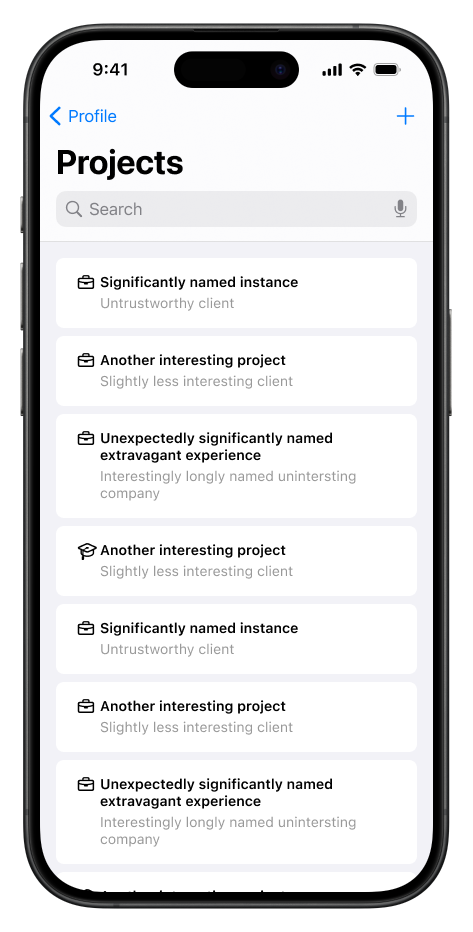
\includegraphics[width=6cm]{projects.png}
		\caption{Seznam}
		\label{fig:project-list}
	\end{subfigure}
	\hspace{2cm}
	\begin{subfigure}[b]{0.4\textwidth}
		\centering
		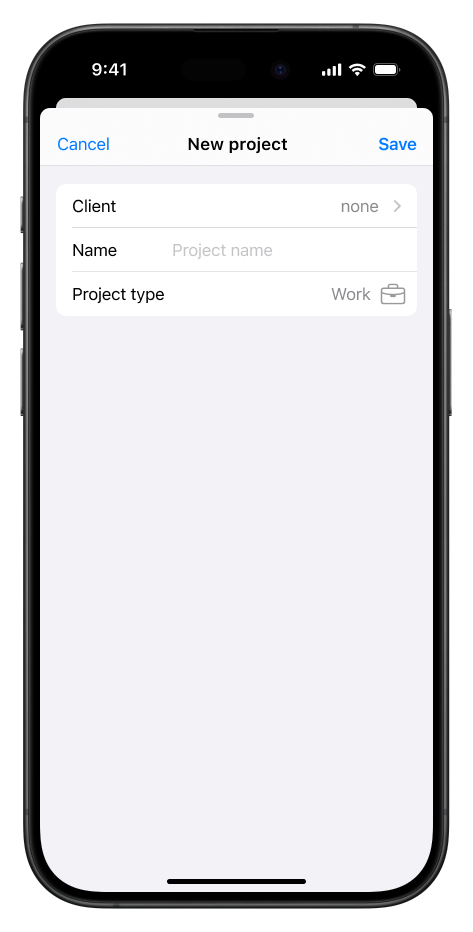
\includegraphics[width=6cm]{new-project.png}
		\caption{Nový projekt}
		\label{fig:new-project}
	\end{subfigure}
	\caption{Projekty}
	\label{fig:projects}
\end{figure}

%---------------------------------------------------------------
\subsection{Integrace}
%---------------------------------------------------------------

Jedním z~cílů práce je stanovit požadavky pro integraci spouštěčů měření času, dále požadavky na integraci aplikace s~existujícími systémy pro měření času, a tyto požadavky v~aplikaci implementovat. Tyto dva typy integrací lze rozdělit do skupin \emph{import} (integrace se spouštěči) a \emph{export} (integrace s~existujícími systémy).

%---------------------------------------------------------------
\subsubsection{Import}
%---------------------------------------------------------------

V~sekci \ref{tracking-triggers} byly popsány teoretické možnosti, s~jakými spouštěči by aplikace šla propojit.

Prvním typem spouštěčů měření času byly fyzické spouštěče, tedy nějaké fyzické formy ovladače. Z~uvedených příkladů v~analýze byl pouze jeden, který by uměl uskutečnit napojení na aplikaci napřímo, a to \emph{TTIMEFLIP} \cite{timeflip}, který poskytuje protokol pro BLE komunikaci. Implementace BLE komunikace s~hardwarovým produktem je ale poměrně komplexní záležitost, která byla začleněna nad rámec rozsahu této práce, která se už takto věnuje návrhu a implementaci celé platformy pro měření odpracovaného času. Implementace tohoto typu komunikace tedy může být podnětem pro budoucí rozšíření aplikace.

Důležité ale je, aby na takové rozšíření byla aplikace dobře připravená, a aby minimálně poskytovala veřejné API umožňující se z~jakéhokoli budoucího konfigurovatelného hardwarového řešení na aplikaci napojit.










































